%%%%%%%%%%%%%%%%%%%%%%%%%%%%%%%%%%%%%%%%%
% Journal Article
% LaTeX Template
% Version 2.0 (February 7, 2023)
%
% This template originates from:
% https://www.LaTeXTemplates.com
%
% Author:
% Vel (vel@latextemplates.com)
%
% License:
% CC BY-NC-SA 4.0 (https://creativecommons.org/licenses/by-nc-sa/4.0/)
%
% NOTE: The bibliography needs to be compiled using the biber engine.
%
%%%%%%%%%%%%%%%%%%%%%%%%%%%%%%%%%%%%%%%%%

%----------------------------------------------------------------------------------------
%	PACKAGES AND OTHER DOCUMENT CONFIGURATIONS
%----------------------------------------------------------------------------------------

\documentclass[
	a4paper, % Paper size, use either a4paper or letterpaper
	10pt, % Default font size, can also use 11pt or 12pt, although this is not recommended
	% unnumberedsections, % Commented to enable section numbering
	twoside, % Two side traditional mode where headers and footers change between odd and even pages, comment this option to make them fixed
	draft, % skips compiling images, which take FOREVER. toggle this on and off to see complete version
]{LTJournalArticle}

\addbibresource{3F3_FTR_zl559.bib} % BibLaTeX bibliography file

\usepackage{amsmath} % For align environment, \text, \implies

\runninghead{Random Variables and Random Number Generation} % A shortened article title to appear in the running head

\footertext{3F3 Full Technical Report} % Text to appear in the footer

\setcounter{page}{1} % The page number of the first page

%----------------------------------------------------------------------------------------
%	TITLE SECTION
%----------------------------------------------------------------------------------------

\title{Random Variables and Random Number Generation} % Article title

% Authors are listed in a comma-separated list with superscript numbers indicating affiliations
\author{%
	Liu Zihe\textsuperscript{1}\thanks{CRSID: zl559. Date: 30th November 2025}
}

% Affiliations are output in the \date{} command
\date{\footnotesize\textsuperscript{\textbf{1}}University of Cambridge}

% Full-width abstract
\renewcommand{\maketitlehookd}{%
	\begin{abstract}
		\noindent This report explores random number generation and density estimation techniques. We compare histogram and kernel density estimation (KDE) methods, demonstrating their trade-offs in accuracy and smoothness. Probability transformations using the Jacobian formula are applied to derive distributions for linear and quadratic functions of normal random variables. The inverse CDF method is implemented to generate exponential random variates. Finally, the alpha-stable distribution is explored, demonstrating heavy-tailed random variable generation with varying stability and skewness parameters.
	\end{abstract}
}

%----------------------------------------------------------------------------------------

\begin{document}

\maketitle % Output the title section

%----------------------------------------------------------------------------------------
%	ARTICLE CONTENTS
%----------------------------------------------------------------------------------------

\section{Introduction}

Random number generation is fundamental to Monte Carlo methods, statistical simulation, and probabilistic modelling. This report investigates the generation and characterisation of random variables, addressing four core topics: (1) density estimation via histograms and kernel density estimation (KDE), (2) probability transformations using the Jacobian formula, (3) the inverse CDF method for generating non-uniform random variables, and (4) the $\alpha$-stable distribution for modelling heavy-tailed phenomena.

Section~\ref{sec:uniform_normal} compares histogram and KDE methods for density estimation, analysing their theoretical convergence properties and practical trade-offs. The multinomial distribution provides the statistical foundation for understanding histogram bin count variability. Section~\ref{sec:functions} applies the Jacobian transformation formula to derive distributions of linear and quadratic functions of Gaussian random variables. Section~\ref{sec:inverse_cdf} develops the inverse CDF method, demonstrating exponential variate generation and proving key properties of Monte Carlo estimators. Finally, Section~\ref{sec:stable} explores the $\alpha$-stable distribution, characterising its heavy-tailed behaviour and relationship to the Gaussian distribution.

%------------------------------------------------

\section{Uniform and Normal Random Variables}
\label{sec:uniform_normal}

\subsection{Kernel Density Estimation}

The kernel density estimator is defined as
\begin{equation}
	\hat{p}(x) = \frac{1}{N}\sum_{i=1}^{N} \frac{1}{\sigma}\mathcal{K}\left(\frac{x - x^{(i)}}{\sigma}\right)
\end{equation}
where $N$ is the number of samples, $x^{(i)}$ are the observed data points, $\mathcal{K}(u)$ is the kernel function, and $\sigma$ is the bandwidth. The Gaussian kernel is:
\begin{equation}
	\mathcal{K}_{\text{Gauss}}(u) = \frac{1}{\sqrt{2\pi}}\exp\left(-\frac{u^2}{2}\right)
\end{equation}
resulting in the KDE:
\begin{equation}
	\hat{p}(x) = \frac{1}{N\sigma}\sum_{i=1}^{N}\exp\left(-\frac{(x - x^{(i)})^2}{2\sigma^2}\right)
\end{equation}

\subsection{Histogram and KDE of Gaussian Random Numbers}

\begin{figure*} % Full width figure
	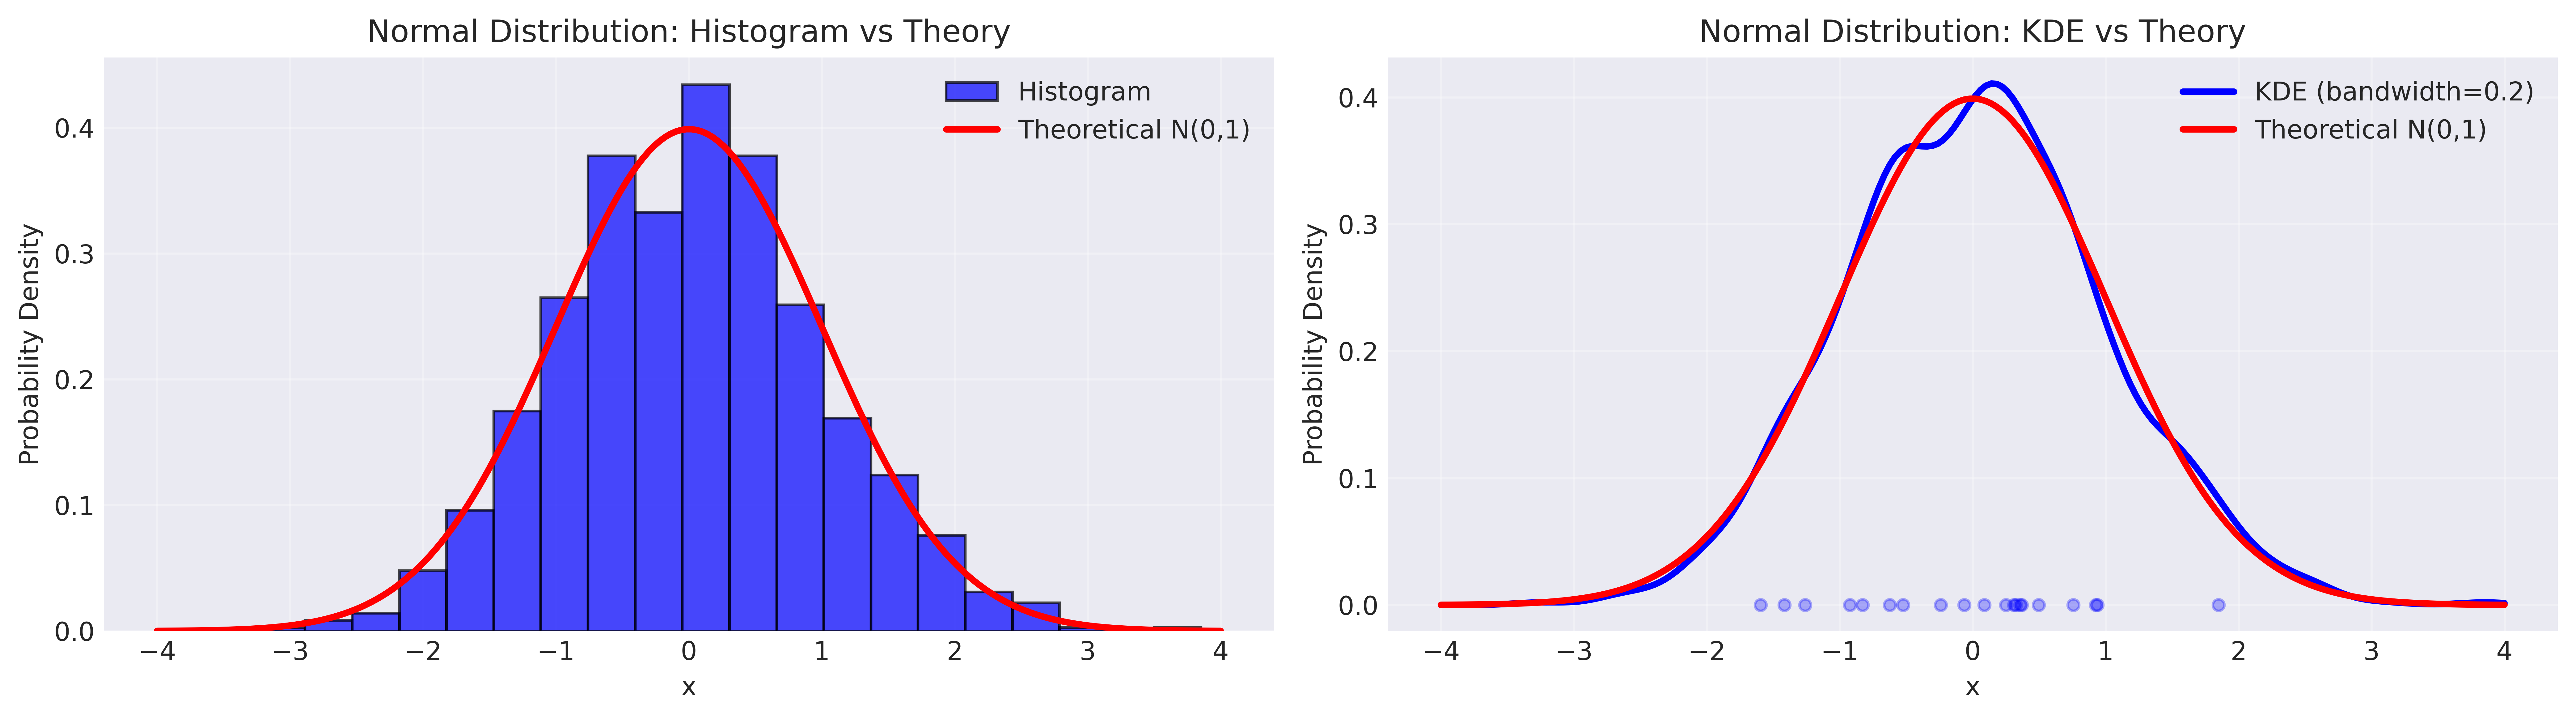
\includegraphics[width=\linewidth]{img/normal_histogram_kde.png}
	\caption{Normal distribution: histogram (left) and KDE (right) compared with theoretical $\mathcal{N}(0,1)$ PDF. The histogram exhibits discontinuities at bin boundaries while KDE ($\sigma=0.2$) produces a smooth estimate.}
	\label{fig:normal}
\end{figure*}

The histogram (blue bars) and KDE (blue curve) both capture the bell-shaped Gaussian profile. The histogram exhibits discontinuities at bin boundaries while the KDE produces a smooth estimate that closely follows the theoretical PDF (red curve).

\subsection{Histogram and KDE of Uniform Random Numbers}

\begin{figure*} % Full width figure
	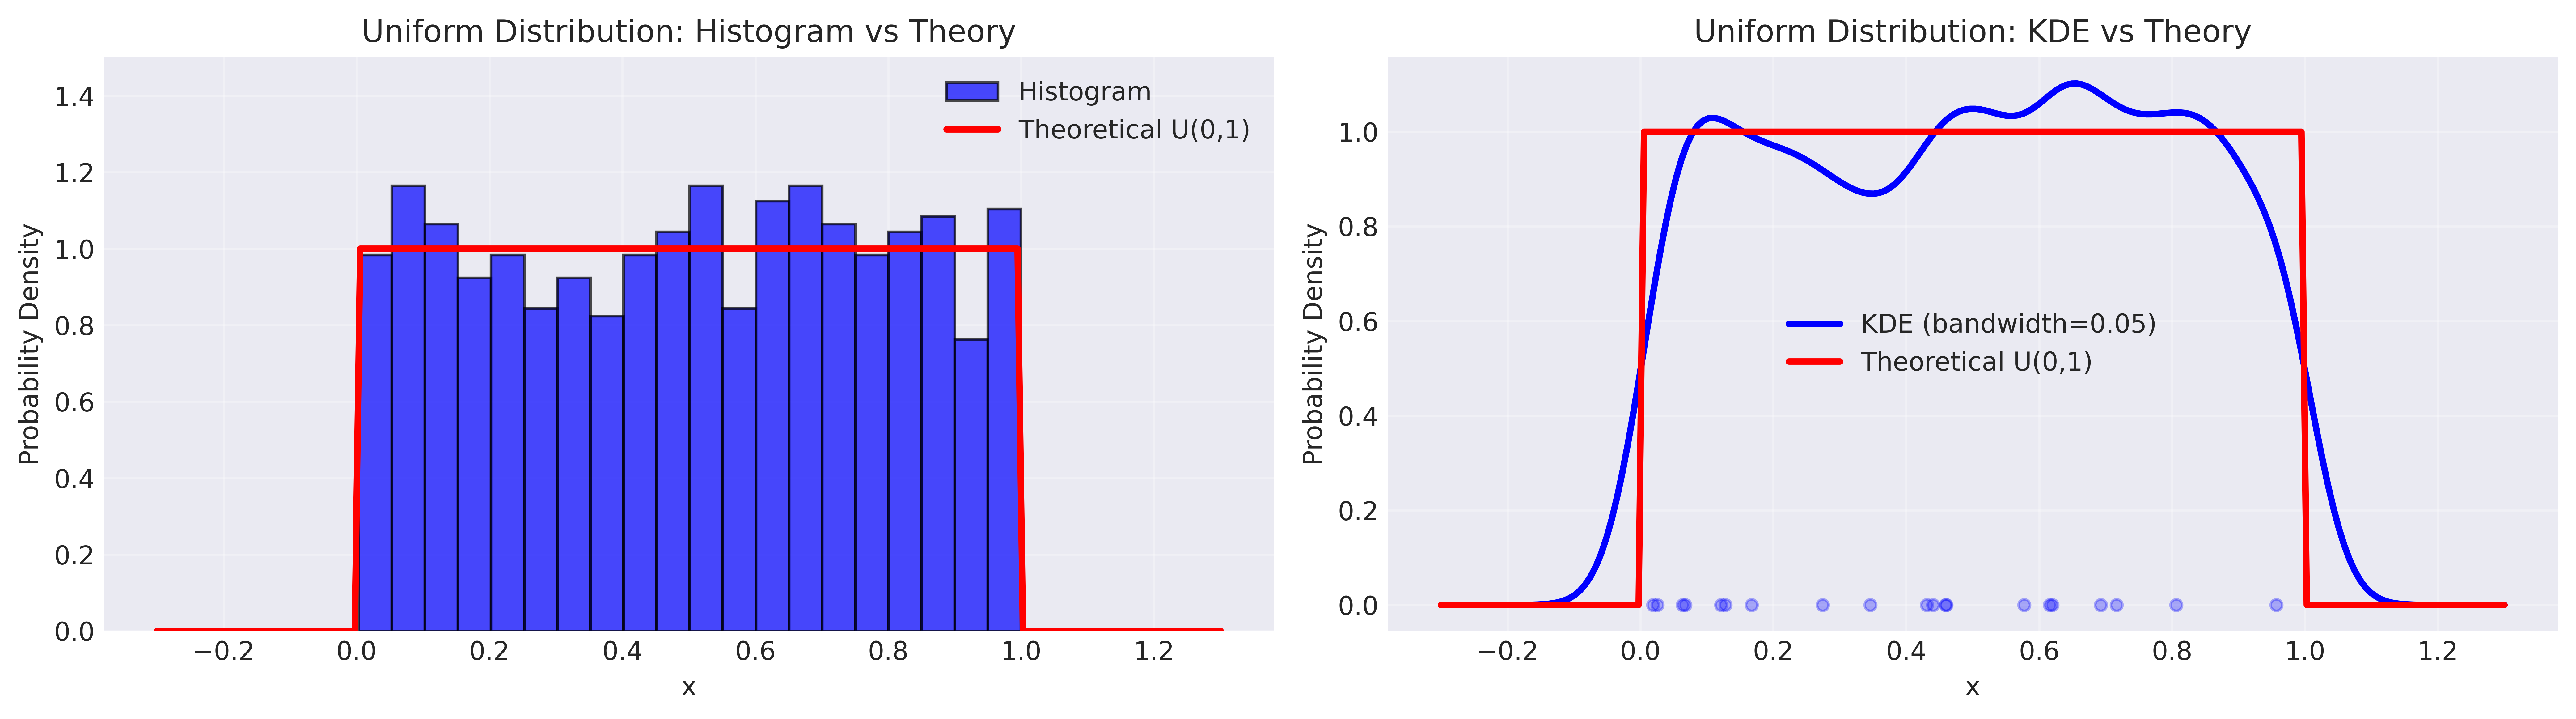
\includegraphics[width=\linewidth]{img/uniform_histogram_kde.png}
	\caption{Uniform distribution: histogram (left) and KDE (right) compared with theoretical $\mathcal{U}(0,1)$ PDF. KDE extends beyond $[0,1]$ due to boundary effects.}
	\label{fig:uniform}
\end{figure*}

The histogram shows approximately equal heights across bins, consistent with uniform density. The KDE ($\sigma=0.05$) is smoother but extends beyond $[0,1]$ due to boundary effects.

\subsection{Comparison of Methods}

Both methods have similar bias-variance structure but differ in asymptotic convergence. From statistical theory \autocite{UW_STAT425}:

\textbf{Histogram:} Optimal convergence rate $O(N^{-2/3})$

\textbf{KDE:} Optimal convergence rate $O(N^{-4/5})$ (faster)

\begin{table}[h] % Single column table
	\caption{Comparison of histogram and KDE methods.}
	\centering
	\footnotesize
	\begin{tabular}{@{}lcc@{}}
		\toprule
		\textbf{Aspect} & \textbf{Histogram} & \textbf{KDE}  \\
		\midrule
		Visual Form     & Discrete bars      & Smooth curve  \\
		Interpretation  & Bin counts         & Smoothed est. \\
		Param. Sens.    & High               & Lower         \\
		Boundary        & Respects           & May exceed    \\
		Convergence     & $O(N^{-2/3})$      & $O(N^{-4/5})$ \\
		Comp. Cost      & Trivial            & $O(N)$        \\
		\bottomrule
	\end{tabular}
	\label{tab:comparison}
\end{table}

\textbf{Histogram advantages:} Directly represents sample counts per bin (intuitive), respects finite support of distributions, computationally simple.

\textbf{Histogram disadvantages:} Sensitive to bin width and position, artificial discontinuities between bins.

\textbf{KDE advantages:} Smooth, continuous estimate revealing density structure, superior convergence rate, less sensitive to bandwidth selection.

\textbf{KDE disadvantages:} Less intuitive, boundary effects for finite support distributions, computationally more expensive.

\subsection{Theoretical Analysis of Uniform Density}

When histogramming $N$ samples from $\mathcal{U}(0,1)$ into $J$ bins, each bin has width $\delta = 1/J$ and probability $p_j = 1/J$. Each marginal count follows:
\begin{equation}
	n_j \sim \text{Binomial}\left(N, p_j = \frac{1}{J}\right)
\end{equation}

Therefore:
\begin{align}
	E[n_j]          & = \frac{N}{J}             \\
	\text{Var}(n_j) & = \frac{N(J-1)}{J^2}      \\
	\sigma_{n_j}    & = \frac{\sqrt{N(J-1)}}{J}
\end{align}

The coefficient of variation is $\text{CV} = \sqrt{(J-1)/N} \approx \sqrt{J/N}$. As $N \to \infty$, CV $\to 0$, so histogram estimates become increasingly reliable.

\begin{figure*} % Full width figure
	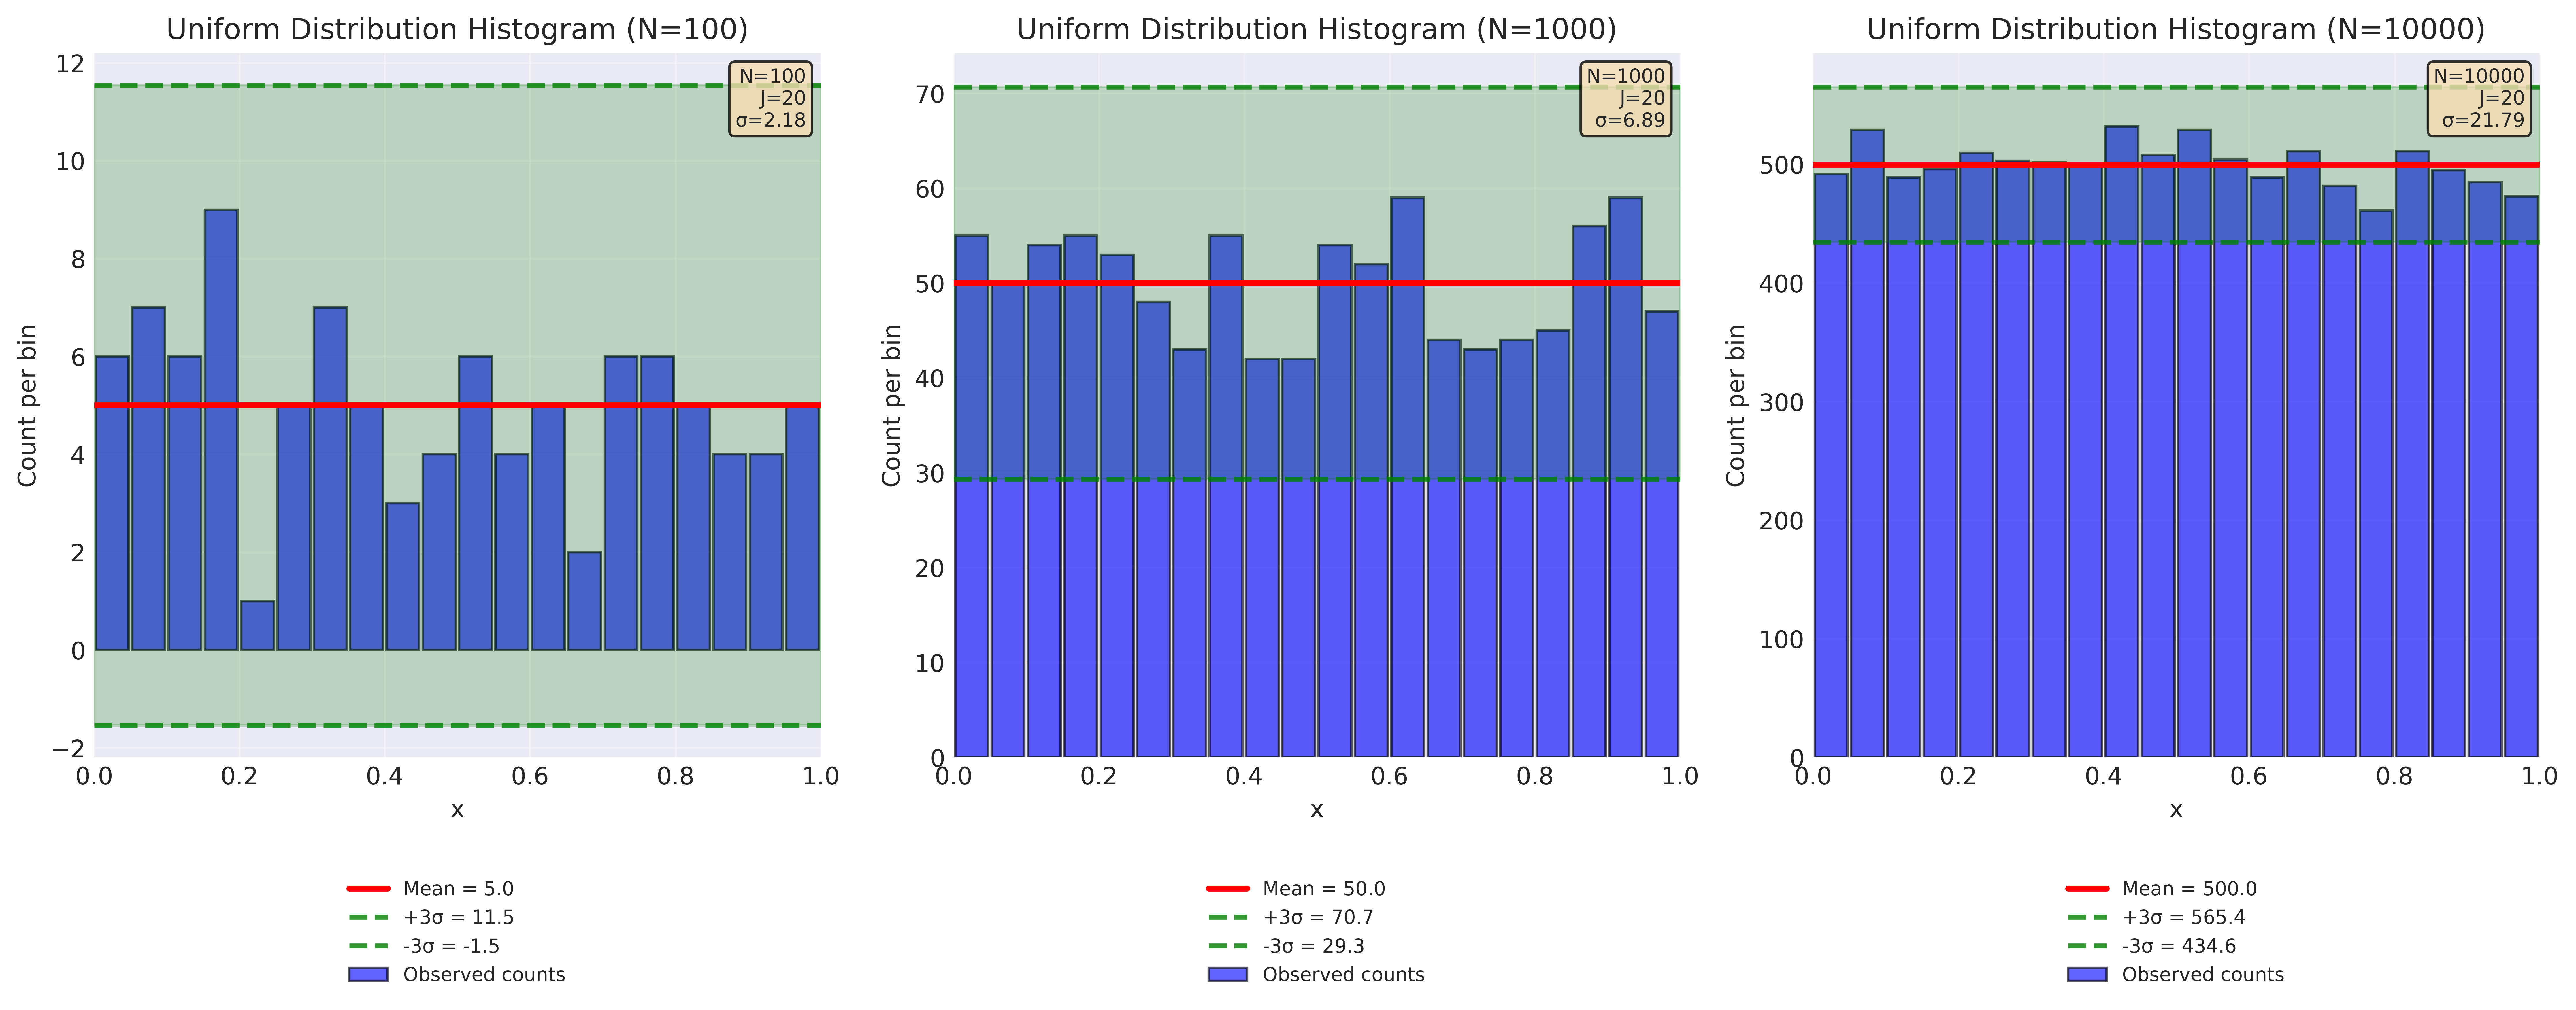
\includegraphics[width=\linewidth]{img/multinomial_bounds.png}
	\caption{Histograms for $N=100, 1000, 10000$ with theoretical mean (red) and $\pm 3\sigma$ bounds (green). As $N$ increases, relative scatter decreases proportionally to $1/\sqrt{N}$.}
	\label{fig:multinomial}
\end{figure*}

The histogram results demonstrate good agreement with theory:
\begin{enumerate}
	\item \textbf{Bin Count Distribution:} Expected mean $E[n_j] = N/J$ closely matches observed counts across all $N$ values.
	\item \textbf{Confidence Bounds:} Approximately 95--100\% of bins fall within $\pm 3\sigma$ bounds, consistent with the $\sim 99.7\%$ theoretical expectation from CLT.
	\item \textbf{Increasing Reliability:} As $N$ increases, relative scatter decreases proportionally to $1/\sqrt{N}$.
\end{enumerate}

\subsection{Multinomial Distribution}

The multinomial distribution describes the probability of observing counts $(n_1, n_2, \ldots, n_J)$ when $N$ independent samples are distributed into $J$ bins, where each sample falls into bin $j$ with probability $p_j$:
\begin{equation}
	P(n_1, \ldots, n_J) = \frac{N!}{n_1! n_2! \cdots n_J!} p_1^{n_1} p_2^{n_2} \cdots p_J^{n_J}
\end{equation}

Each sample is an independent trial. For a specific sample to land in bin $j$, the probability is $p_j$. Since all $N$ samples are independent, the probability of a specific sequence of outcomes is the product of individual probabilities $p_1^{n_1} \times p_2^{n_2} \times \cdots \times p_J^{n_J}$. If exactly $n_j$ samples land in bin $j$, these contribute a factor of $p_j^{n_j}$.

The factorial coefficient counts the number of distinct arrangements that yield the same bin counts. Consider $N$ labelled samples: the number of ways to choose which $n_1$ samples go to bin 1, then which $n_2$ of the remaining go to bin 2, and so forth, is:
\begin{equation}
	\binom{N}{n_1}\binom{N-n_1}{n_2}\cdots\binom{n_J}{n_J} = \frac{N!}{n_1! n_2! \cdots n_J!}
\end{equation}
This multinomial coefficient counts the number of ways to partition $N$ distinct objects into $J$ groups of sizes $n_1, \ldots, n_J$.

\subsection{Multinomial Analysis for Normal Distribution}

For normally distributed data $X \sim \mathcal{N}(0, 1)$, the bin probabilities $p_j$ are non-uniform. They must be calculated using the CDF:
\begin{equation}
	p_j = \Phi(b_{j+1}) - \Phi(b_j)
\end{equation}
where $\Phi(x)$ is the standard normal CDF and $[b_j, b_{j+1})$ defines bin $j$.

Central bins (near $x = 0$) have high probability because the PDF is peaked there, while edge bins (large $|x|$) have low probability due to exponential decay. The variance of bin counts depends on bin probability:
\begin{equation}
	\text{Var}(n_j) = N p_j (1 - p_j)
\end{equation}

This variance is maximised when $p_j = 0.5$ (intermediate) and minimised when $p_j \to 0$ or $p_j \to 1$. For histograms of normal data, edge bins have the highest \textit{relative} uncertainty $\sigma_{n_j}/E[n_j] = \sqrt{(1-p_j)/(Np_j)}$, making histogram estimates in the tails less reliable.

\begin{figure*}
	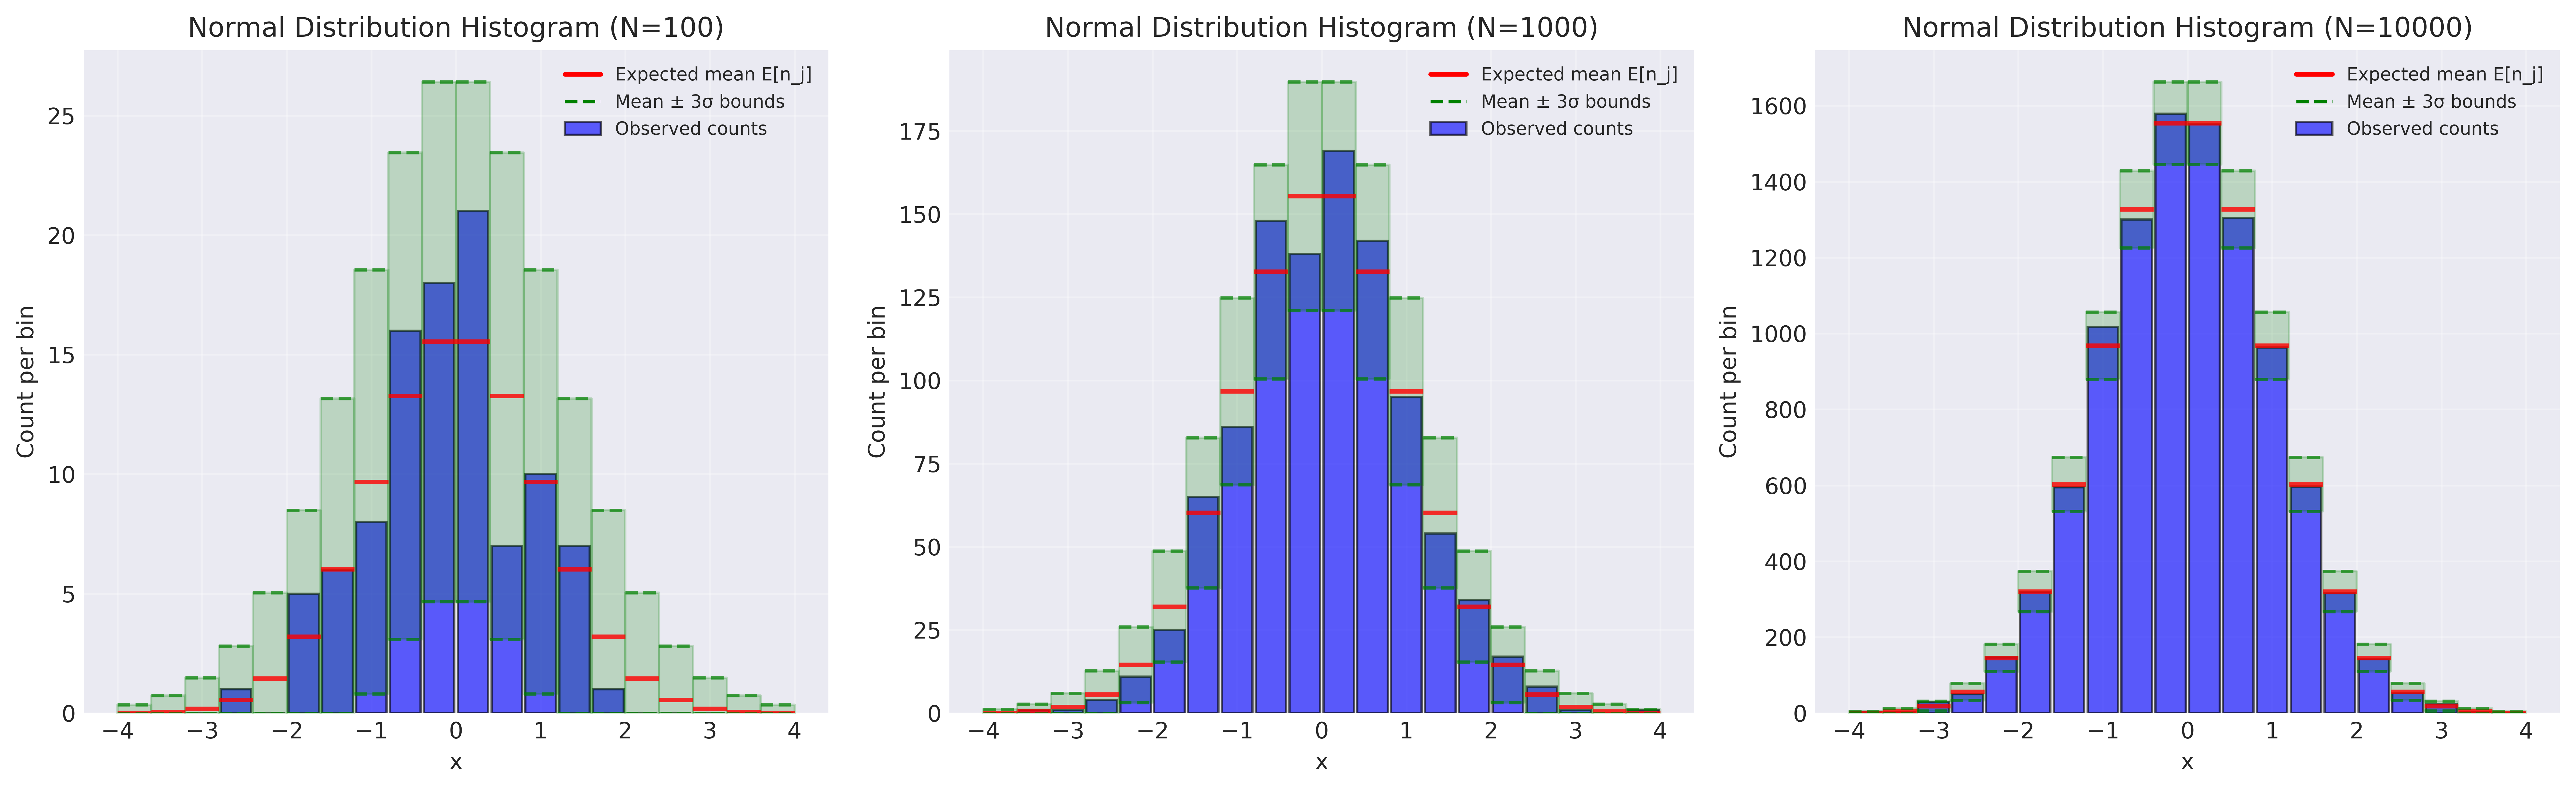
\includegraphics[width=\linewidth]{img/normal_multinomial_bounds.png}
	\caption{Histograms of normal samples for $N=100, 1000, 10000$ with theoretical mean (red) and $\pm 3\sigma$ bounds (green). Unlike uniform data, the bounds vary across bins due to non-uniform bin probabilities.}
	\label{fig:normal_multinomial}
\end{figure*}

%------------------------------------------------

\section{Functions of Random Variables}
\label{sec:functions}

\subsection{Linear Transformation}

For $x \sim \mathcal{N}(0,1)$ and $y = ax + b$, the inverse is $x = (y-b)/a$ with Jacobian $|dx/dy| = 1/|a|$. Applying the transformation formula:
\begin{align}
	p(y) & = p(x)\left|\frac{dx}{dy}\right| \nonumber                                                   \\
	     & = \frac{1}{\sqrt{2\pi}}\exp\left(-\frac{(y-b)^2}{2a^2}\right) \cdot \frac{1}{|a|}  \nonumber \\
	     & = \frac{1}{\sqrt{2\pi a^2}}\exp\left(-\frac{(y-b)^2}{2a^2}\right) \nonumber                  \\
	     & = \mathcal{N}(y|b, a^2)
\end{align}

This demonstrates that a linear transformation of standard normal produces $\mathcal{N}(\mu, \sigma^2)$ with $\mu = b$ and $\sigma^2 = a^2$. Any normal distribution can be generated from $\mathcal{N}(0,1)$ using $Y = \sigma X + \mu$.

\begin{figure}[h] % Single column figure
	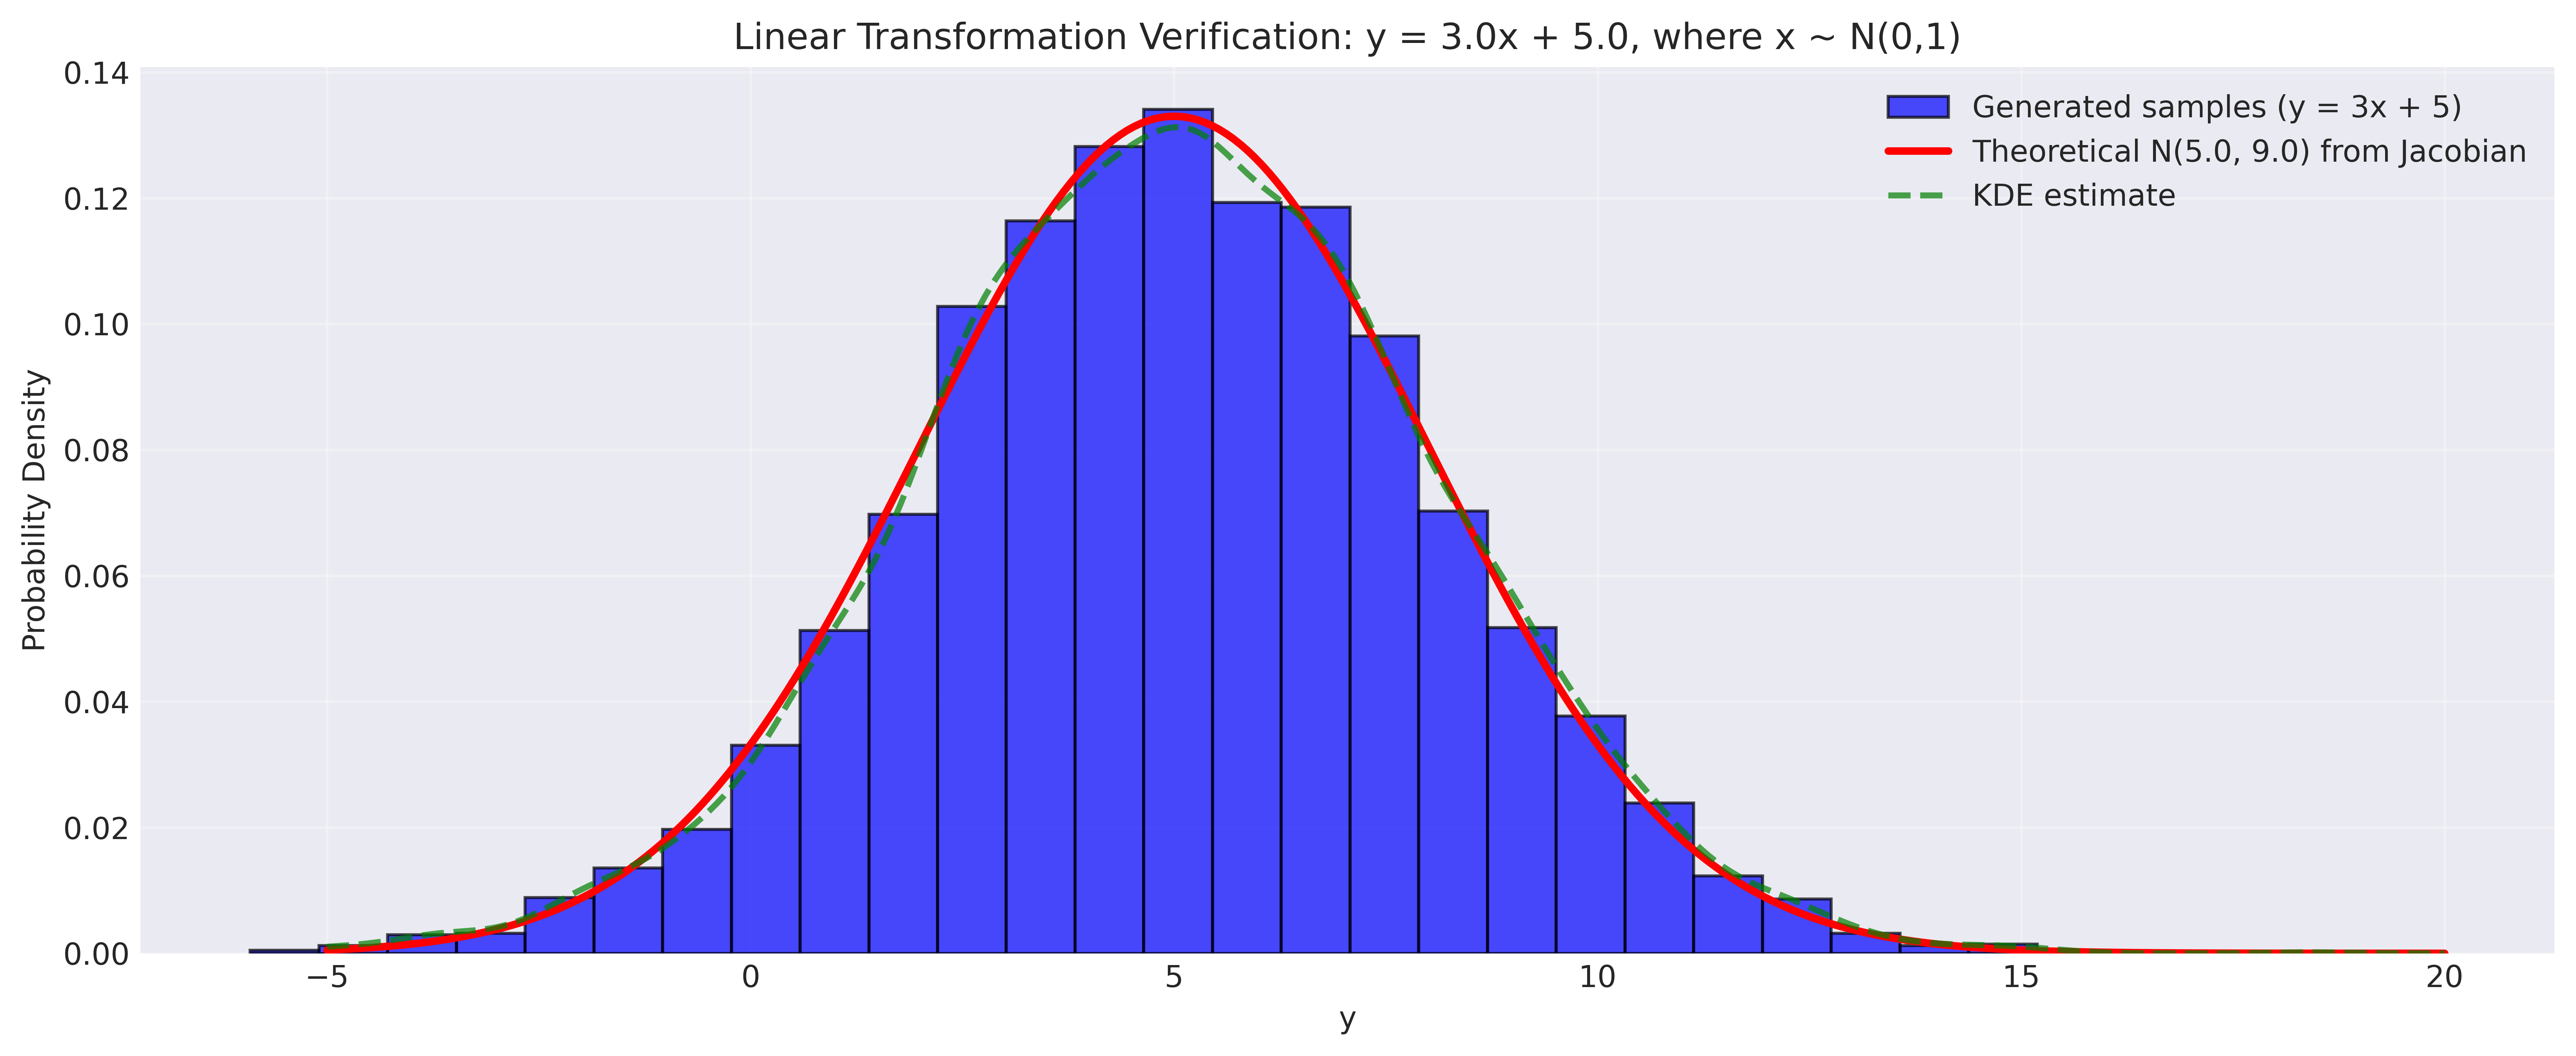
\includegraphics[width=\linewidth]{img/linear_transform_verification.png}
	\caption{Verification of linear transformation $y = 3x + 5$ where $x \sim \mathcal{N}(0,1)$. The histogram matches theoretical $\mathcal{N}(5, 9)$.}
	\label{fig:linear}
\end{figure}

\subsection{Quadratic Transformation}

For $x \sim \mathcal{N}(0,1)$ and $y = x^2$ ($y \geq 0$), there are two inverses: $x_1(y) = \sqrt{y}$ and $x_2(y) = -\sqrt{y}$. The Jacobian is $|dx/dy| = 1/(2\sqrt{y})$. Applying the formula:
\begin{align}
	p(y) & = 2 \cdot \frac{1}{\sqrt{2\pi}}\exp\left(-\frac{y}{2}\right) \cdot \frac{1}{2\sqrt{y}} \nonumber \\
	     & = \frac{1}{\sqrt{2\pi y}}\exp\left(-\frac{y}{2}\right), \quad y \geq 0
\end{align}

This is the chi-squared distribution with 1 degree of freedom, $\chi^2_1$.

\begin{figure}[h] % Single column figure
	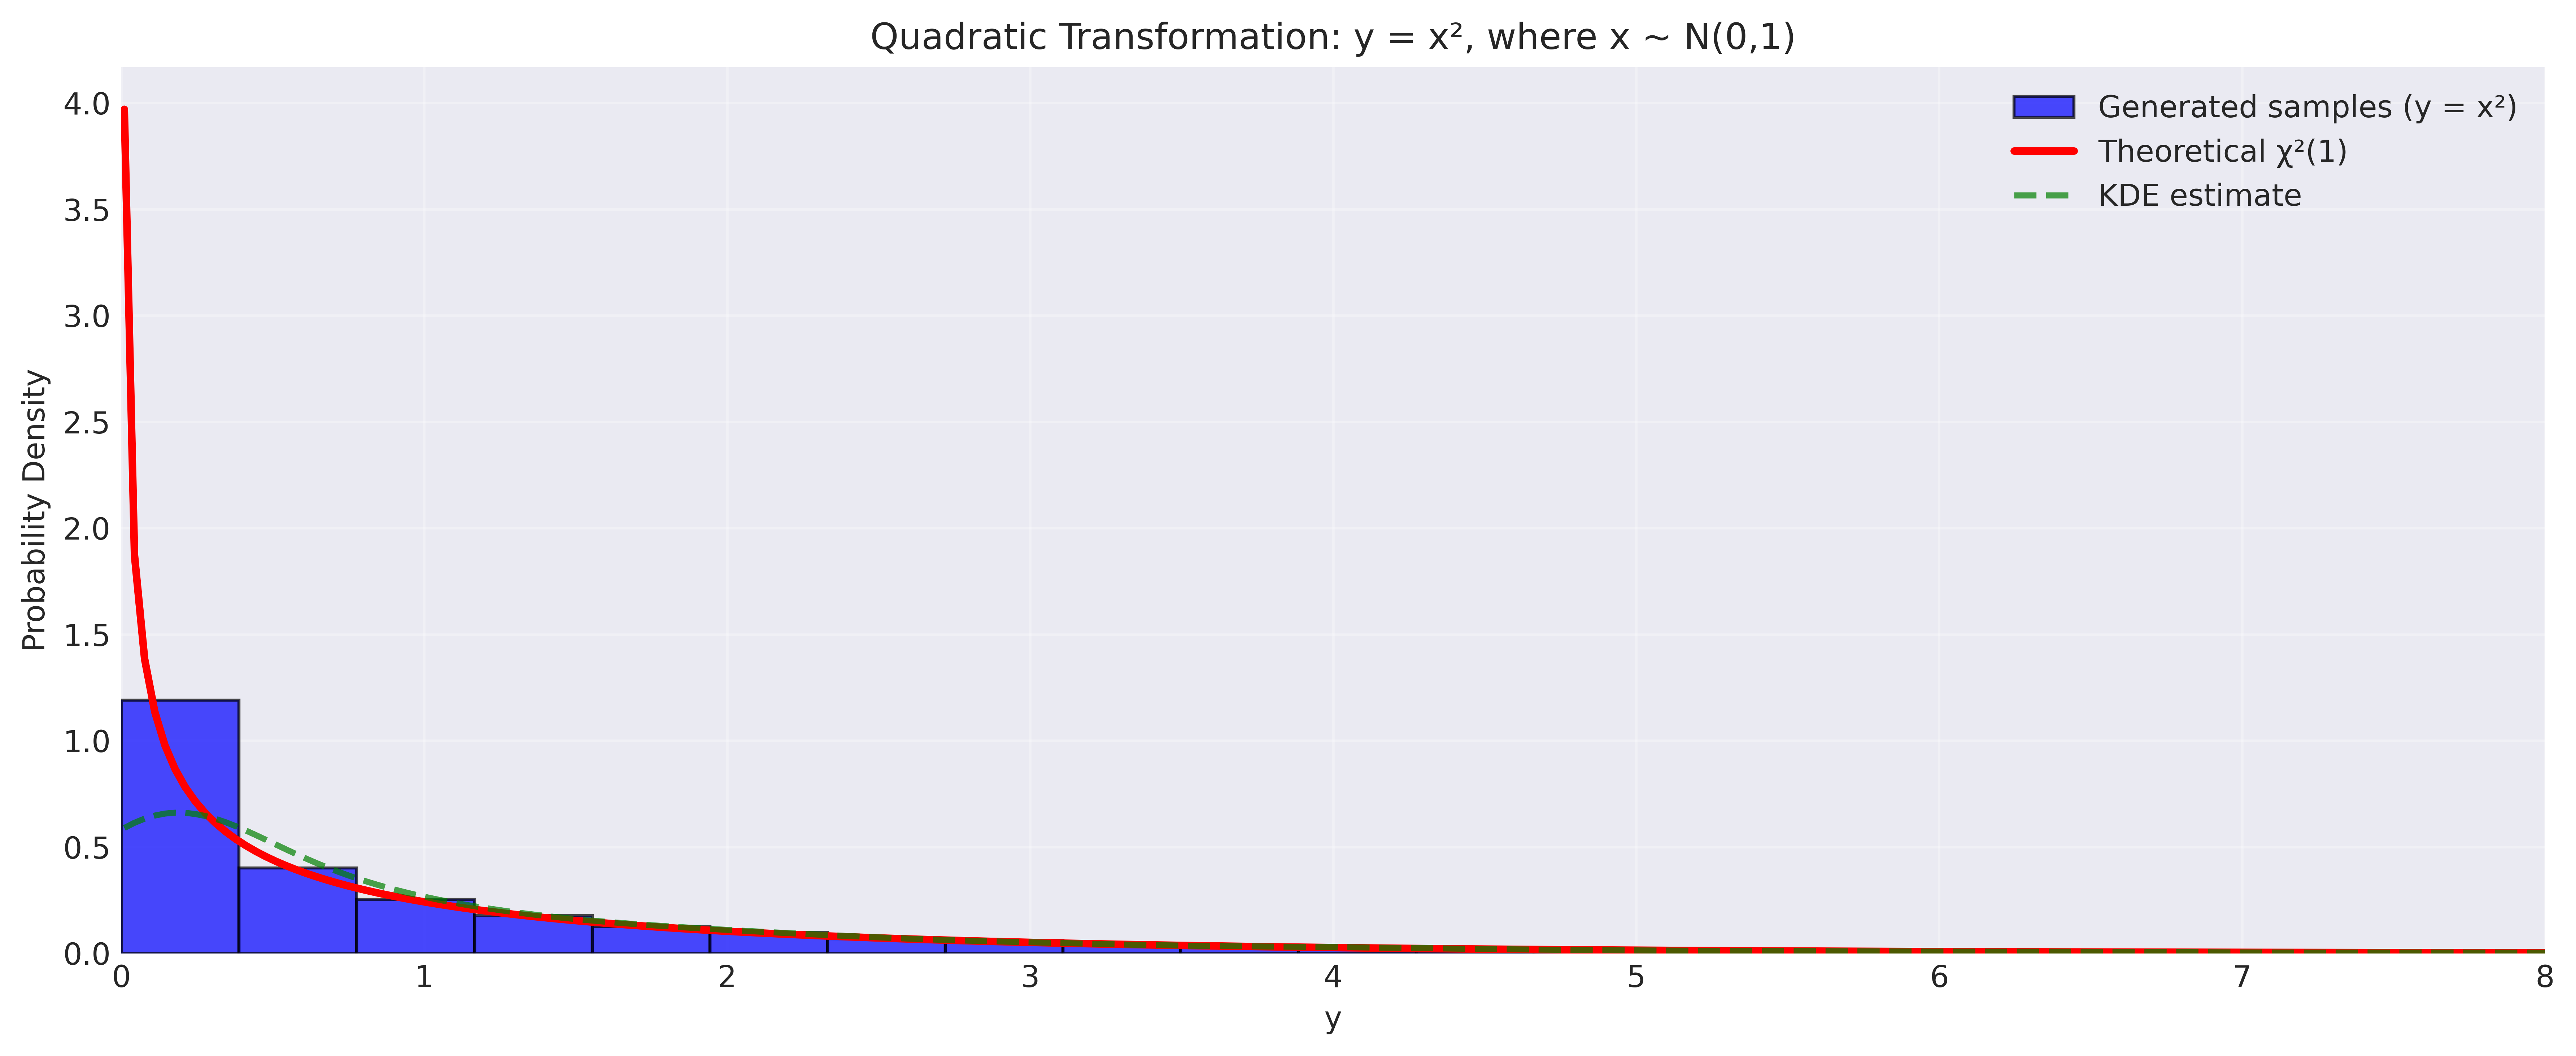
\includegraphics[width=\linewidth]{img/quadratic_transform_verification.png}
	\caption{Verification of quadratic transformation $y = x^2$. Sample mean $\approx 1.0$ and variance $\approx 2.0$ match theoretical $\chi^2_1$ moments.}
	\label{fig:quadratic}
\end{figure}

%------------------------------------------------

\section{Inverse CDF Method}
\label{sec:inverse_cdf}

\subsection{Theory}

If $U \sim \mathcal{U}(0,1)$ and $Y = F^{-1}(U)$ where $F$ is any CDF, then $Y$ has distribution with CDF $F$. The algorithm:
\begin{enumerate}
	\item Generate $u^{(i)} \sim \mathcal{U}(0,1)$
	\item Compute $y^{(i)} = F^{-1}(u^{(i)})$
\end{enumerate}

\subsection{Exponential Distribution}

For the exponential distribution with PDF $p(y) = \exp(-y)$ for $y \geq 0$:

\textbf{CDF:}
\begin{equation}
	F(y) = \int_{0}^{y} \exp(-t)\, dt = 1 - \exp(-y)
\end{equation}

\textbf{Inverse CDF:} Solving $u = F(y)$ for $y$:
\begin{align}
	u = 1 - \exp(-y) \implies y = -\ln(1 - u) = F^{-1}(u)
\end{align}

Since $(1-u) \sim \mathcal{U}(0,1)$ when $u \sim \mathcal{U}(0,1)$, we can use $F^{-1}(u) = -\ln(u)$.

\subsection{Implementation}

\begin{verbatim}
def generate_exponential(n, mean=1.0):
    u = np.random.rand(n)
    return -mean * np.log(u)
\end{verbatim}

\begin{figure*} % Full width figure
	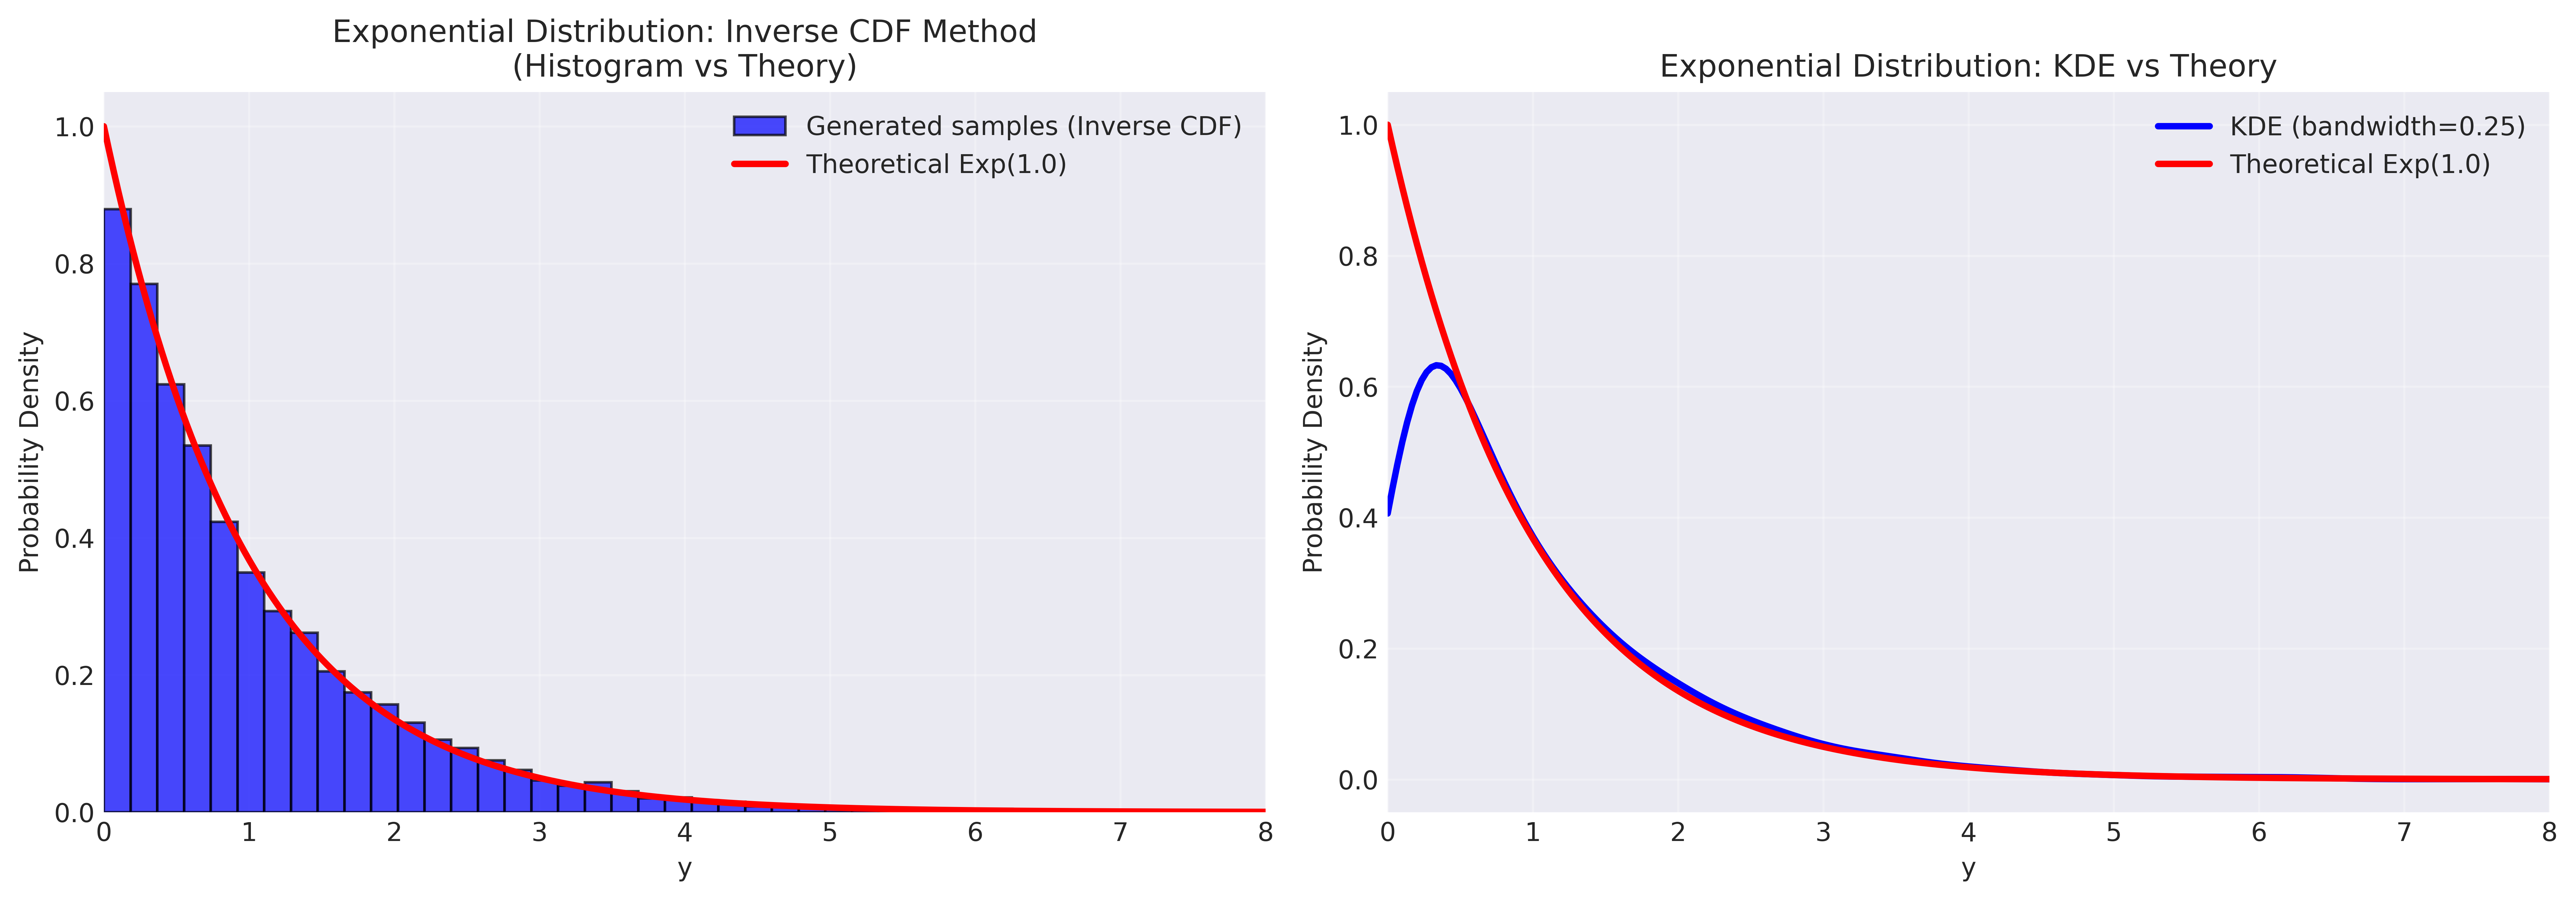
\includegraphics[width=\linewidth]{img/exponential_inverse_cdf.png}
	\caption{Exponential distribution via inverse CDF method. Histogram (left) matches theoretical PDF. KDE (right) shows boundary effects: peak underestimated ($\approx 0.65$ vs 1.0) due to Gaussian kernels extending into $y < 0$.}
	\label{fig:exponential}
\end{figure*}

The histogram shows excellent agreement with the theoretical exponential density. The KDE exhibits boundary effects near $y = 0$ where Gaussian kernels extend beyond the valid support $[0,\infty)$.

\subsection{Monte Carlo Estimation of Moments}

Given $N$ i.i.d.\ samples $y^{(1)}, \ldots, y^{(N)}$ from a distribution with mean $\mu$ and variance $\sigma^2$, we define the sample mean estimator:
\begin{equation}
	\hat{\mu} = \frac{1}{N}\sum_{i=1}^{N} y^{(i)}
\end{equation}

For the exponential distribution with $\lambda = 1$, the theoretical mean is $E[Y] = 1$ and variance is $\text{Var}(Y) = 1$. Experimental verification with $N = 10000$ samples yields $\hat{\mu} \approx 1.00$ and $\hat{\sigma}^2 \approx 1.00$, confirming the inverse CDF method correctly generates exponential variates.

\subsection{Unbiasedness of the Mean Estimator}

The sample mean $\hat{\mu}$ is an unbiased estimator of the true mean $\mu$. To prove this, we compute the expectation over all possible samples:
\begin{align}
	E[\hat{\mu}] & = E\left[\frac{1}{N}\sum_{i=1}^{N} y^{(i)}\right] \nonumber \\
	             & = \frac{1}{N}\sum_{i=1}^{N} E[y^{(i)}] \nonumber            \\
	             & = \frac{1}{N} \cdot N \cdot \mu = \mu
\end{align}
where we used linearity of expectation and that each $y^{(i)}$ has the same mean $\mu$.

\subsection{Variance of the Mean Estimator}

The variance of $\hat{\mu}$ determines how quickly the estimate converges to the true mean:
\begin{align}
	\text{Var}(\hat{\mu}) & = \text{Var}\left(\frac{1}{N}\sum_{i=1}^{N} y^{(i)}\right) \nonumber    \\
	                      & = \frac{1}{N^2} \text{Var}\left(\sum_{i=1}^{N} y^{(i)}\right) \nonumber \\
	                      & = \frac{1}{N^2} \cdot N\sigma^2 = \frac{\sigma^2}{N}
\end{align}
where we used independence of samples (variance of sum equals sum of variances).

The standard error is $\text{SE}(\hat{\mu}) = \sigma/\sqrt{N}$, implying that doubling the number of samples only reduces the error by a factor of $\sqrt{2}$. This $O(1/\sqrt{N})$ convergence rate is fundamental to Monte Carlo methods.

\subsection{Monte Carlo Convergence}

\begin{figure*}
	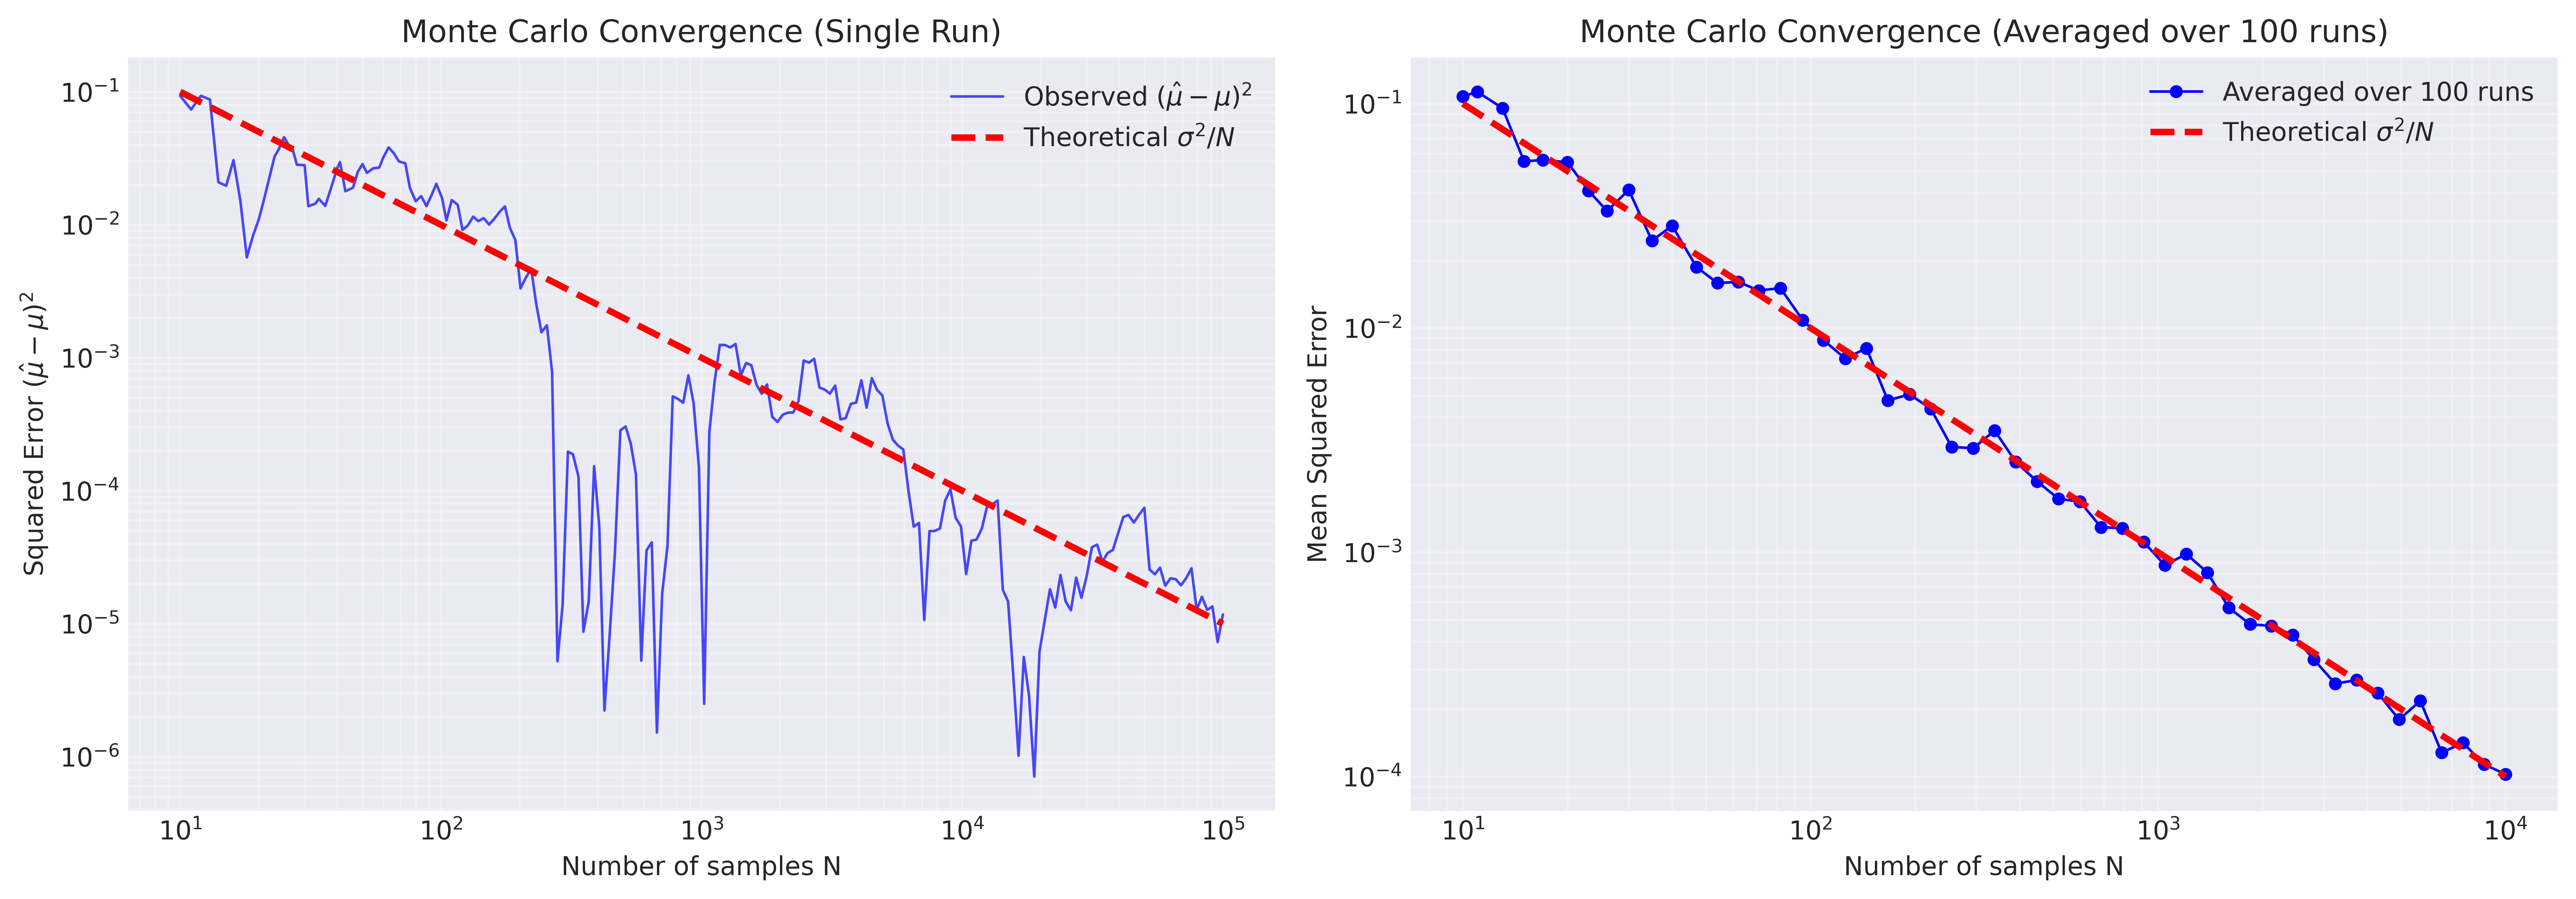
\includegraphics[width=\linewidth]{img/mc_convergence.png}
	\caption{Monte Carlo convergence for exponential distribution. Left: Single run showing squared error $(\hat{\mu} - \mu)^2$ versus $N$ with theoretical variance $\sigma^2/N$ (dashed). Right: Averaged squared error over 100 runs confirms $1/N$ decay rate.}
	\label{fig:mc_convergence}
\end{figure*}

Figure~\ref{fig:mc_convergence} demonstrates the $1/N$ variance decay. While individual runs show fluctuations, the averaged squared error closely follows the theoretical $\sigma^2/N$ bound. This confirms that the Monte Carlo estimator is consistent: as $N \to \infty$, $\hat{\mu} \to \mu$ by the Law of Large Numbers.

%------------------------------------------------

\section{Alpha-Stable Distribution}
\label{sec:stable}

\subsection{Generation Algorithm}

The $\alpha$-stable distribution models heavy-tailed phenomena in communications and signal processing. To generate samples with $\alpha \in (0,2)$, $\alpha \neq 1$ and $\beta \in [-1,+1]$:

\begin{enumerate}
	\item Calculate auxiliary parameters:
	      \begin{align}
		      b & = \frac{1}{\alpha}\arctan\left(\beta\tan\frac{\pi\alpha}{2}\right) \\
		      s & = \left(1 + \beta^2\tan^2\frac{\pi\alpha}{2}\right)^{1/(2\alpha)}
	      \end{align}

	\item Generate $U \sim \mathcal{U}(-\pi/2, +\pi/2)$ and $V \sim \mathcal{E}(1)$

	\item Calculate:
	      \begin{equation}
		      X = s \frac{\sin(\alpha(U + b))}{(\cos U)^{1/\alpha}}\left(\frac{\cos(U - \alpha(U + b))}{V}\right)^{\frac{1-\alpha}{\alpha}}
	      \end{equation}
\end{enumerate}

\subsection{Implementation}

\begin{verbatim}
def generate_stable(alpha, beta, n):
    b = (1/alpha) * np.arctan(
        beta * np.tan(np.pi*alpha/2))
    s = (1 + beta**2 * np.tan(
        np.pi*alpha/2)**2)**(1/(2*alpha))
    U = np.random.uniform(
        -np.pi/2, np.pi/2, n)
    V = np.random.exponential(1.0, n)
    num = np.sin(alpha*(U+b)) / \
          np.cos(U)**(1/alpha)
    den = (np.cos(U-alpha*(U+b))/V) \
          **((1-alpha)/alpha)
    return s * num * den
\end{verbatim}

\begin{figure*} % Full width figure
	\includegraphics[width=\linewidth]{img/stable_distribution_grid.png}
	\caption{Alpha-stable distributions for $\alpha = 0.5$ (top, heavy tails) and $\alpha = 1.5$ (bottom, lighter tails) with varying $\beta$ (skewness). Heavy-tailed distributions ($\alpha = 0.5$) produce extreme outliers requiring plot clipping.}
	\label{fig:stable}
\end{figure*}

\subsection{Parameter Interpretation}

\textbf{Stability parameter $\alpha \in (0,2)$:} Controls tail heaviness. At $\alpha = 0.5$, tails are extremely heavy with massive outliers. At $\alpha = 1.5$, tails are lighter but still heavier than Gaussian. As $\alpha \to 2$, the distribution approaches Gaussian.

\textbf{Skewness parameter $\beta \in [-1,+1]$:} Controls asymmetry. At $\beta = 0$, the distribution is symmetric. Positive $\beta$ produces right skewness; negative $\beta$ produces left skewness.

\subsection{Tail Probability Analysis}

A key distinction between $\alpha$-stable and Gaussian distributions lies in their tail behaviour. For $\alpha$-stable distributions with $\alpha < 2$, the tail probability follows a power law:
\begin{equation}
	P(|X| > t) \sim c \cdot t^{-\alpha} \quad \text{as } t \to \infty
\end{equation}

In contrast, the Gaussian has exponentially decaying tails: $P(|Z| > t) \sim e^{-t^2/2}/(t\sqrt{\pi})$.

\begin{table}[h]
	\caption{Tail probabilities $P(|X| > t)$ for different distributions.}
	\centering
	\footnotesize
	\begin{tabular}{@{}lccc@{}}
		\toprule
		\textbf{Distribution}            & $t=0$ & $t=3$  & $t=6$              \\
		\midrule
		Gaussian ($\alpha = 2$)          & 1.0   & 0.0027 & $2 \times 10^{-9}$ \\
		$\alpha$-stable ($\alpha = 1.5$) & 1.0   & 0.11   & 0.04               \\
		$\alpha$-stable ($\alpha = 0.5$) & 1.0   & 0.30   & 0.21               \\
		\bottomrule
	\end{tabular}
	\label{tab:tail_probs}
\end{table}

Table~\ref{tab:tail_probs} demonstrates the dramatic difference: at $t = 6$, the Gaussian tail probability is essentially zero ($\sim 10^{-9}$), while the $\alpha$-stable with $\alpha = 0.5$ still has $P(|X| > 6) \approx 0.21$. This explains why heavy-tailed distributions produce extreme outliers.

\begin{figure*}
	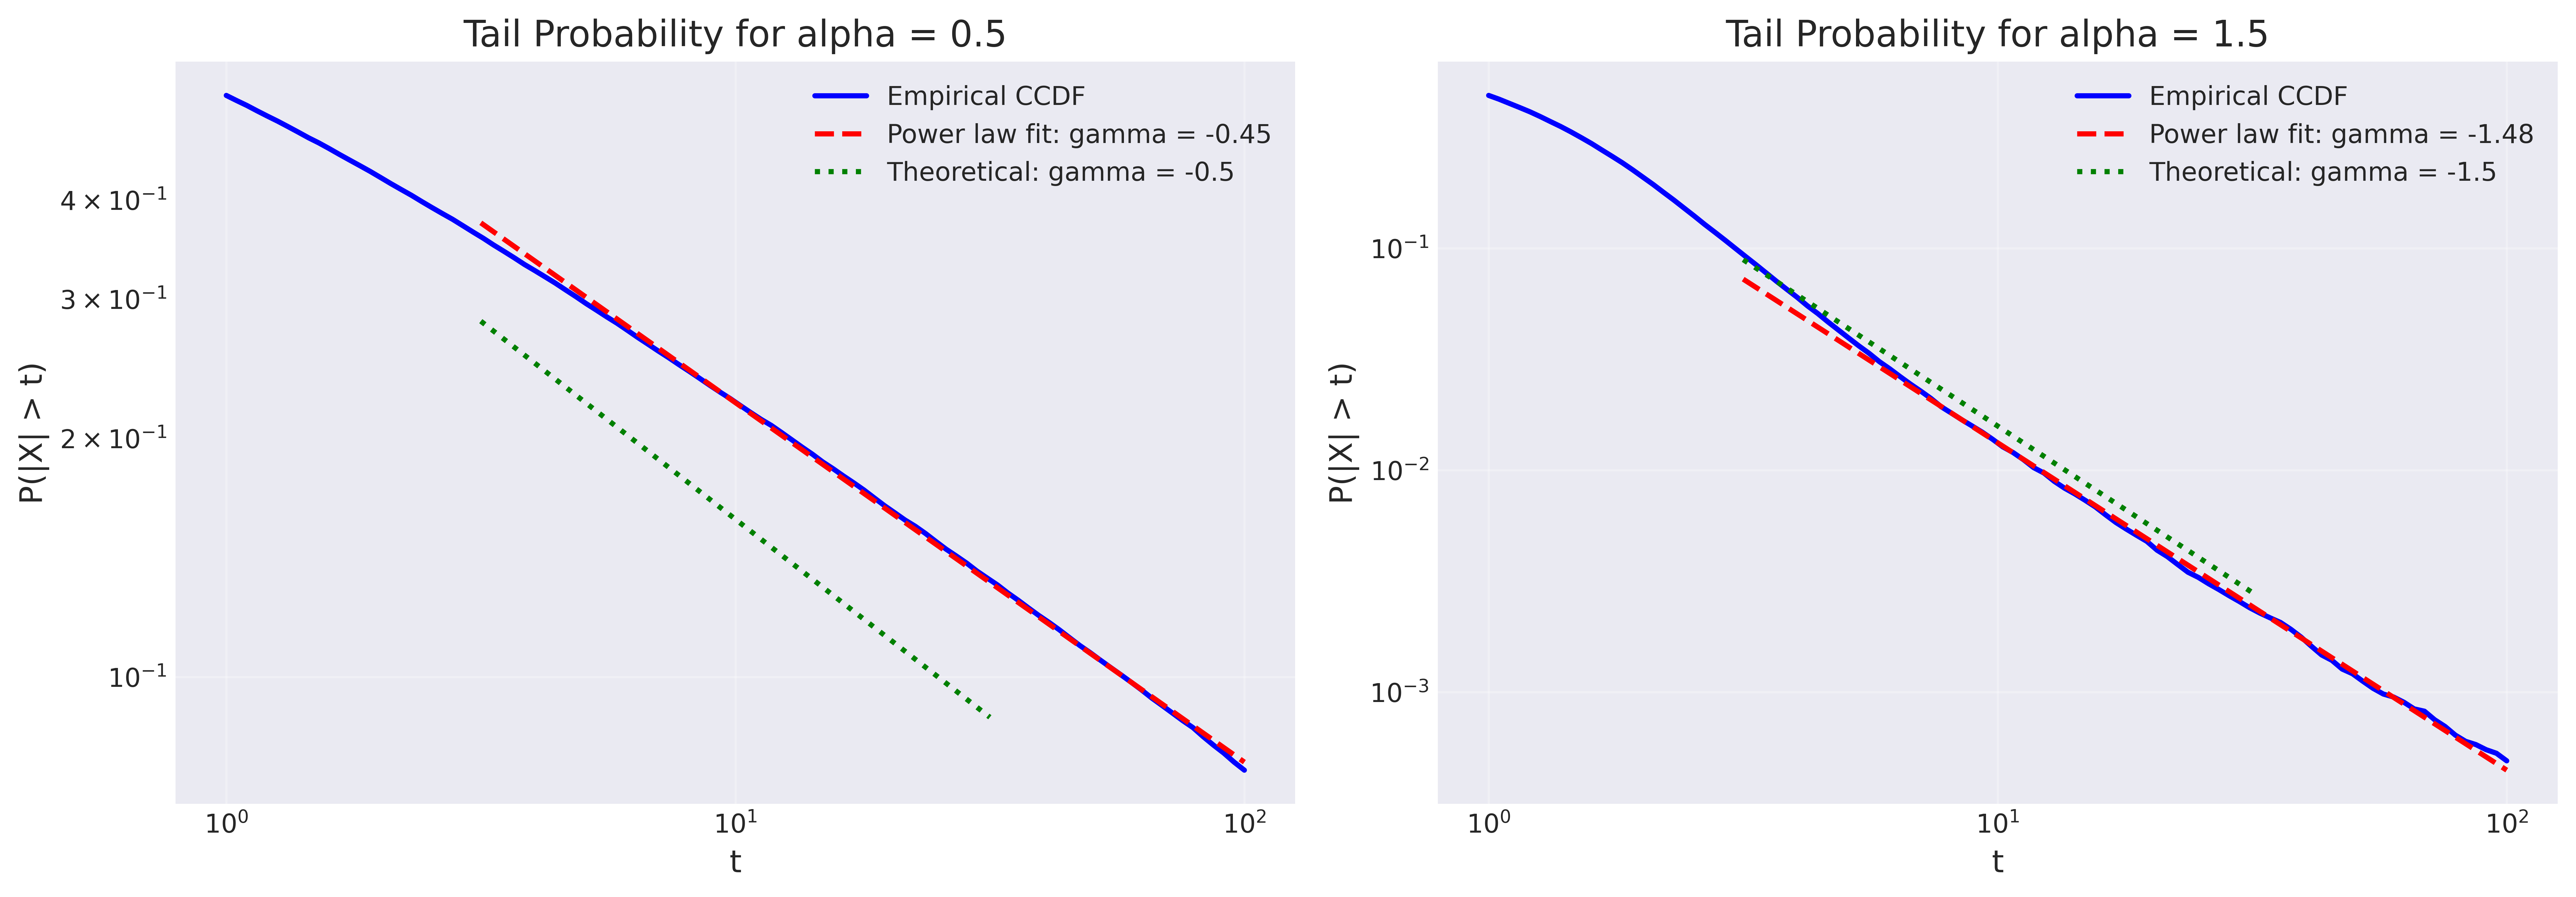
\includegraphics[width=\linewidth]{img/power_law_tail_fit.png}
	\caption{Power law tail fitting for $\alpha$-stable distributions. Log-log plots of $P(|X| > t)$ versus $t$ show linear decay with slope $\gamma \approx -\alpha$, confirming the theoretical prediction.}
	\label{fig:tail_fit}
\end{figure*}

Figure~\ref{fig:tail_fit} confirms that $P(|X| > t) \propto t^{\gamma}$ with $\gamma \approx -\alpha$. Linear regression on the log-log plot yields $\gamma = -0.50$ for $\alpha = 0.5$ and $\gamma = -1.50$ for $\alpha = 1.5$, validating the general formula $\gamma = -\alpha$.

\subsection{Convergence to Gaussian as $\alpha \to 2$}

As the stability parameter $\alpha$ approaches 2, the $\alpha$-stable distribution converges to a Gaussian. This transition involves fundamental changes in the distribution's properties:

\textbf{Tail behaviour:} For $\alpha < 2$, tails follow a power law with infinite variance. At $\alpha = 2$, tails decay exponentially with finite variance.

\textbf{Characteristic function:} The $\alpha$-stable characteristic function is $\phi(t) = \exp(-|t|^\alpha)$. As $\alpha \to 2$, this approaches $\exp(-t^2)$, the Gaussian characteristic function.

\textbf{Central Limit Theorem connection:} The Gaussian is the unique stable distribution ($\alpha = 2$) that arises as the limit of standardised sums by the CLT. For $\alpha < 2$, sums of i.i.d.\ heavy-tailed variables converge to $\alpha$-stable distributions instead.

\begin{figure*}
	\includegraphics[width=\linewidth]{img/stable_gaussian_convergence.png}
	\caption{Convergence of $\alpha$-stable to Gaussian as $\alpha \to 2$. For $\alpha = 0.5$, the distribution has extremely heavy tails. As $\alpha$ increases through 1.5, 1.7, 1.9, 1.99, the distribution progressively approaches the Gaussian (red curve).}
	\label{fig:stable_convergence}
\end{figure*}

Figure~\ref{fig:stable_convergence} illustrates this convergence visually. At $\alpha = 1.99$, the histogram is nearly indistinguishable from the Gaussian reference, while at $\alpha = 0.5$ the heavy tails produce a sharply peaked distribution with frequent extreme values.

%----------------------------------------------------------------------------------------
%	CONCLUSION
%----------------------------------------------------------------------------------------

\section{Conclusion}

This report investigated random number generation and density estimation techniques across four main topics.

\textbf{Density estimation:} Histogram and KDE methods offer complementary trade-offs. Histograms are intuitive, respect bounded support, and directly represent bin counts, while KDE provides smoother estimates with faster asymptotic convergence ($O(N^{-4/5})$ versus $O(N^{-2/3})$). The multinomial distribution provides the theoretical foundation for histogram bin count variability, with the factorial terms counting distinct arrangements and the power terms arising from independent trials.

\textbf{Jacobian transformations:} The change-of-variables formula enables derivation of transformed variable distributions. Linear transformations of standard normals yield general Gaussians ($y = ax + b \Rightarrow \mathcal{N}(b, a^2)$), while quadratic transformations produce chi-squared distributions ($y = x^2 \Rightarrow \chi^2_1$).

\textbf{Inverse CDF method:} This general framework generates samples from any distribution with invertible CDF, as demonstrated for the exponential distribution. The Monte Carlo mean estimator $\hat{\mu}$ is unbiased ($E[\hat{\mu}] = \mu$) with variance $\text{Var}(\hat{\mu}) = \sigma^2/N$, yielding the characteristic $O(1/\sqrt{N})$ convergence rate.

\textbf{Alpha-stable distributions:} These model heavy-tailed phenomena with power-law tail decay $P(|X| > t) \sim t^{-\alpha}$, in contrast to the exponential decay of Gaussians. The stability parameter $\alpha$ controls tail heaviness, with $\alpha \to 2$ recovering the Gaussian as a limiting case. This connection to the Central Limit Theorem highlights the Gaussian as the unique finite-variance stable distribution.

%----------------------------------------------------------------------------------------
%	 REFERENCES
%----------------------------------------------------------------------------------------

\printbibliography % Output the bibliography

%----------------------------------------------------------------------------------------

\end{document}
